\documentclass[tikz,margin=0pt,dvipsnames,rgb]{standalone}


\usepackage{amsmath,amssymb,amsfonts}
\usetikzlibrary{calc,
fit,
shapes.misc,
shapes.geometric,
arrows.meta,
fadings,
matrix,
chains,
scopes,
positioning}

\usepackage{pgfplots}
\usepackage{pgfplotstable}
\pgfplotsset{compat=1.18}



\usepackage[]{fontspec}

\setmainfont{Latin Modern Roman}
\setmonofont{Latin Modern Math}
\renewcommand{\textsc}[1]{{\fontfamily{lmr}\selectfont \scshape #1}}

\usepackage[]{bm}

\makeatletter
\@ifundefined{fromRoot}{\newcommand{\fromRoot}[1]{../../#1}}{}

\def\input@path{{../..}{..}{.}{./svg}{./pgfplots}{./tikzpicture}}
%or: \def\input@path{{/path/to/folder/}{/path/to/other/folder/}}
\makeatother

\newcommand{\ra}[1]{\renewcommand{\arraystretch}{#1}}

\newcommand*{\gf}[1]{\acrshort{gf}($#1$)}%
\newcommand*{\mpn}[1]{\bm{P}_{#1}}%
\newcommand*{\pn}[1]{%
  \ifthenelse{\equal{#1}{}}{$\mpn{0}$}{$\mpn{#1}$}%
}%

\newcommand*{\pk}[3]{%
  \ifthenelse{\equal{#1}{#2}}{\textcolor{red}{\phantom{.}$p_0$\phantom{.}}}{\phantom{.}$p_#3$\phantom{.}}%
}%


\newcommand*{\placeholderreg}{\includegraphics[width=\linewidth, height=.25\textheight, keepaspectratio = true]{figures/certified_xilinx.png}}%
\newcommand*{\placeholder}[1]{\includegraphics[#1]{figures/certified_xilinx.png}}%

\newcommand*{\snr}{\acrshort{snr}}%
\newcommand*{\snrs}{\acrshortpl{snr}}%

\newcommand*{\mpd}[0]{p_\Delta}%
\newcommand*{\mpo}[0]{p_\omega}%
\newcommand*{\pd}[0]{$\mpd$}%
\newcommand*{\po}[0]{$\mpo$}%
\newcommand*{\mpfa}[0]{\mathcal{P}_{fa}}%
\newcommand*{\mpmd}[0]{\mathcal{P}_{md}}%
\newcommand*{\pfa}[0]{\acrshort{pfa}}%
\newcommand*{\pmd}[0]{\acrshort{pmd}}%
\newcommand*{\mnorm}[1]{\mathcal{L}_{#1}}%
\newcommand*{\norm}[1]{$\mnorm{#1}$}%
\newcommand*{\fft}{\acrshort{fft}}%
\newcommand*{\mfft}[1]{\mathcal{F}(#1)}%
\newcommand*{\mifft}[1]{\mathcal{F}^{-1}(#1)}%
\newcommand*{\ts}{\acrshort{ts}}%

\newcommand*{\cpp}[1]{C\textrm{++#1}}%
\newcommand*{\na}{\textrm{\textcolor{SlateGray4}{N/A}}}%

\newcommand*{\vect}[1]{\bm{#1}}%
\newcommand*{\mat}[1]{\bm{\mathrm{#1}}}%

\newcommand*{\task}[1]{\mathcal{T}_{#1}}%

\newcommand*{\sdr}{\acrshort{sdr}}%
\newcommand*{\fpga}{\acrshort{fpga}}%

\newcommand*{\rikiki}{\fontsize{4}{6}\selectfont}%



\begin{document}
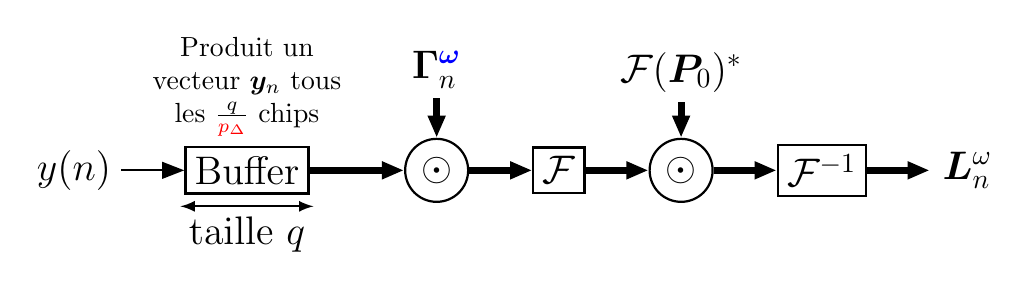
\begin{tikzpicture} [->,
  >={Triangle[width=6pt, length=8pt]},
  auto,
  thick,
  main node/.style={rectangle, fill = white!35, draw,
      align=center},
  every node/.style = {font=\Large},
  ]

  \node [main node,
    draw = none,
    % fill = gray!40!white, 
    % minimum size = 1cm
  ] (input) at (0, 0) {$y(n)$};

  \node [main node,
    draw,
    % fill = gray!40!white, 
    % minimum size = 1cm
    right = .8 cm of input
  ] (pack) {Buffer};

  \node [black,
    font = {\normalsize},
    % fill = gray!40!white, 
    % minimum size = 1cm
    anchor = south,
    align = center
  ] at (pack.north) {Produit un\\vecteur $\vect{y}_n$ tous\\les $\frac{q}{\textcolor{Red}{p_\Delta}}$ chips};

  \draw (input.east) -> (pack.west);
  \draw [latex-latex] ($(pack.south west) + (-.05, -.15)$) -> ($(pack.south east) + (.05, -.15)$)
  node [midway, anchor = north] {taille $q$};

  \node [circle,
    draw,
    % fill = gray!40!white, 
    right = 1.2 cm of pack,
    minimum size = .8 cm
  ] (multf) {};
  \node [circle,
    draw=none,
    % fill = gray!40!white, 
    anchor = center,
    minimum size = .8 cm
  ] at (multf.center) {$\odot$};
  % \draw [-] ($(multf.north west) + (.1, -.1) $) -- ($(multf.south east) + (-.1,  .1) $);
  % \draw [-] ($(multf.south west) + (.1,  .1) $) -- ($(multf.north east) + (-.1, -.1) $);


  % \draw [line width=2.6pt] ($(multf.north) + (0, .5)$) -> (multf.north)
  % node [pos=0, above, align=center] () {$e^{-j\frac{\omega k}{q}}_{(k = 0, 1, \dots, q - 1)}$};
  \node [anchor = south] (gnw) at ($(multf.north) + (0, .5)$) {$\vect{\Gamma}_n^{\textcolor{blue}{\bm{\omega}}}$};

  \draw [line width = 2.6pt] (gnw.south) -> (multf.north);

  \node [main node,
    % fill = gray!40!white, 
    % minimum size = 1.2cm,
    right = .8 cm of multf
  ] (fft) {$\mathcal{F}$};

  \draw [line width=2.6pt] (multf.east) -> (fft.west);

  \node [circle,
    draw,
    % fill = gray!40!white,
    right = .8 cm of fft,
    minimum size = .8 cm
  ] (mult) {};

  \node [circle,
    draw=none,
    % fill = gray!40!white, 
    anchor = center,
    minimum size = .8 cm
  ] at (mult.center) {$\odot$};
  % \draw [-] ($(mult.north west) + (.1, -.1) $) -- ($(mult.south east) + (-.1,  .1) $);
  % \draw [-] ($(mult.south west) + (.1,  .1) $) -- ($(mult.north east) + (-.1, -.1) $);

  % \draw [line width=2.6pt] ($(mult.north) + (0, .5)$) -> (mult.north)
  % node [pos=0, above, align=center] () {$\mathrm{FFT}(\vect{P}_0)$};
  \node [anchor = south, align=center] (fpn) at ($(mult.north) + (0, .45)$) {$\mathcal{F}(\mpn{0})^\ast$};

  \draw  [line width=2.6pt] (fpn.south) -> (mult.north);
  \draw  [line width=2.6pt] (fft.east) -> (mult.west);

  \node [main node,
    % fill = gray!40!white, 
    % minimum size = 1.2cm,
    right = .8 cm of mult
  ] (ifft) {$\mathcal{F}^{-1}$};

  \draw  [line width=2.6pt] (mult.east) -> (ifft.west);

  % \draw  [line width=2.6pt] ($(multf.west) + (-.8, 0)$) ->  (multf.west)
  % node [pos=0, left, align=center] () {$\vect{y}_n$\\(q chips)};
  \draw  [line width=2.6pt] (pack.east) -> (multf.west);

  \draw  [line width=2.6pt] (ifft.east) -> ($(ifft.east) + (.8, 0)$)
  node [pos=1, right, align=center] () {$\vect{L}_n^\omega$};
\end{tikzpicture}

\end{document}
